\documentclass[10pt,a4paper,hidelinks]{article}
\usepackage[utf8]{inputenc}
\usepackage[english]{babel}
\usepackage[T1]{fontenc}

\newcommand{\documentStatus}{DRAFT}


\usepackage{amsmath}
\usepackage{amsfonts}
\usepackage{amssymb}
\usepackage{graphicx}
\usepackage{lmodern}
\usepackage{tikz}
\usetikzlibrary{positioning}
\usepackage{epigraph} 
\usepackage[left=2.5cm,
            right=2.5cm,
            top=2cm,
            bottom=2cm]{geometry}
\usepackage{setspace}
\usepackage{caption}
\usepackage{subcaption}
\usepackage{epigraph}
\usepackage{pdflscape}
\usepackage{pgfplots}

\usepackage{titlesec}
\usepackage{tcolorbox}
\usepackage{background}
\usepackage{url}
\usepackage[pdfauthor={Pierre Jézégou},
            pdftitle={ADS assignement},
            pdfsubject={Word games},
            pdfkeywords={}]{hyperref}
\usepackage{wrapfig}


\backgroundsetup{contents=\documentStatus, color=\watermarkColor}

\usepackage{fancyhdr}
\usepackage{textpos}
\usepackage{sectsty}
\usepackage{xcolor}

\setlength{\parindent}{0pt}

%%%%%%%%%%%%%%% Colors %%%%%%%%%%%%%%%
\subsectionfont{\color{fib_red}}
\subsubsectionfont{\color{fib_red}}
\renewcommand\fbox{\fcolorbox{black}{fib_red!20}}

\definecolor{fib_red}{RGB}{191,21,64}
\definecolor{fib_gray}{RGB}{111,111,111}
\definecolor{blue_upc}{RGB}{52,120,186}

\usepackage{listings}
\lstdefinestyle{mystyle}{
  backgroundcolor=\color{gray!10},
  stringstyle=\color{green!60!black!80},
  keywordstyle=\color{fib_red},
  numberstyle=\tiny\color{fib_gray},
  commentstyle=\color{blue_upc},
  basicstyle=\ttfamily\footnotesize,
  breakatwhitespace=false,         
  breaklines=true,                 
  captionpos=b,                    
  keepspaces=true,                 
  numbers=left,                    
  numbersep=5pt,                  
  showspaces=false,                
  showstringspaces=false,
  showtabs=false,                  
  tabsize=2
}

\lstset{style=mystyle}

\usepackage[Bjornstrup]{fncychap}
\newcommand{\watermarkColor}{red!10}


\onehalfspacing


\newcommand\VRule[1][\arrayrulewidth]{\vrule width #1}
\usepackage{xcolor,colortbl}

\newtcolorbox{mybox}[1]{
    arc=5pt,
    boxrule=0pt,
    colback=#1,
    width=\linewidth,
    halign=left,
}

\newenvironment{framed}[3]{
    \vspace*{0.5em}
    \begin{mybox}{#3!10}
        \textbf{#1} :\hfill \textit{#2}\\
        \hrule\vspace*{1em}
}
{\end{mybox}}

\newenvironment{exercise_description}[1]{
    \begin{framed}{Exercice description}{#1}{orange}
}
{\end{framed}}

\newenvironment{summary}{
    \begin{framed}{Summary}{Section \thesection}{blue}
}
{\end{framed}}

\usepackage{lmodern}
\renewcommand*\familydefault{\sfdefault}


\fancyfoot[R]{\raisebox{-0.5\baselineskip}{
\includegraphics[scale=0.25]{images/logos/upc_logo.jpeg}}}

\begin{document}
\pagestyle{plain}
\backgroundsetup{contents=,color=red!30}
\pagecolor{white}

\begin{center}
    \color{red!50!white}
    \textbf{\huge{STATUT - \documentStatus}}
\end{center}

\vfill

\color{black}
\begin{center}
    % \includegraphics[width=0.5\linewidth]{images/logos/fib.png} \\
    
\includegraphics[height=2cm]{images/logos/upc_logo.jpeg} \\
    \vfill

    \rule{\linewidth}{0.5mm} \\[1cm]
    {\Huge \textsc{\textcolor{fib_red}{Word Games}}}\\[1cm]
    {\Large \textsc{Assignment}}\\[0.4cm]
    {\huge \textsc{\textbf{Advanced data structures}}}\\[1cm]
    {\Large \textsc{Master in Research and Innovation - UPC}}\\[0.4cm]
    \rule{\linewidth}{0.5mm} \\[1.5cm]
\end{center}

\vfill

\textbf{Authors :}
\begin{itemize}
\item Pierre \textsc{Jézégou}\newline
\textit{(Engineering student at École Centrale de Lille, Exchange student at UPC)}
\end{itemize}

\vfill

\newpage
\color{black}
\pagecolor{white}
\pagestyle{fancy}
\tableofcontents

\section{Introduction}
This program implements a trie data structure to store words.
A trie is a tree-like data structure that stores a dynamic set of strings, where each node represents a single character of the string.
The TrieNode class represents the structure of a trie node, which contains information such as its children, whether it marks the end of a word, its value (character), and its depth in the trie.\\

The Trie class implements the operations and building procedure for the trie. It has methods to insert words into the trie and to search for words in the trie.
The program also includes functions to generate TikZ code for visualizing the trie. The \verb|generate_tikz_trie| function generates TikZ code to visualize the trie structure, while the \verb|generate_search_path| function generates TikZ code to visualize the search path for a given word in the trie.
Finally, the program creates an instance of the Trie class, inserts words from a given dictionary into the trie, and generates TikZ code to visualize the trie with a specific search word highlighted.\\

All the source code (programs, documentation and image generators) is available in the GitHub respository dedicated to the project: \url{https://github.com/pierre-jezegou/word-game}\\

For performance testing of algorithms, we use a MacBook Air with the M2 processor. This hardware provides ample computing power to execute our algorithms efficiently, ensuring swift analysis of their performance.

As recommended, this report has been written in \LaTeX.

\section{Word Challenge}
\begin{exercise_description}{Word challenge}
    In Word Challenge the user gives a (multi)set of up to 17 letters, and the program produces all words which can be written using a subset of the given letters. For example, if the user gives the letters \verb|{E,T,F,H,R,R,E,O,E}| the program will write by increasing length and then in alphabetic order all the words that can be built using (some) of these letters, for example, \verb|FOR, HER, ORE, THE, .., HERE, ..., THEREFORE|. The dictionary does only contain words of $\text{length}\geqslant  3$, hence if given $\ell \geqslant 3$ the list of results starts with words of length 3 and ends with words of length $\ell$ (or smaller, if there were no words of length $\ell$ using all given letters). Besides being able to play interactively with the user, the program must give an "automatic mode" in which the program does the following repeatedly:
    \begin{enumerate}
    \item Picks a random word from the dictionary of given length $\ell$
    \item Rearranges its letters randomly
    \item Supplies these letters to the function that generates the list of words which can be built from the given letters
    \end{enumerate}
    In automatic mode the user gives the number of times that the game will be played, and the length $\ell$, and it outputs the average number of words found and the average CPU time that the program takes to "solve" a word of length $\ell$.
\end{exercise_description}


\subsection{Implement \type{trie} data structure}
To begin with, we've chosen to base this exercise on a well-known string structure: tries. This will enable us to store words in a structured way and retrieve them with less complexity (justified later).\\
This structure is based on two classes, \textit{Python}, to model the trie itself (\type{Trie}) and the nodes of the \textit{trie} \type{TrieNode}. Each of these two data structures will be endowed with parameters and methods enabling the job to be solved in an optimal way.


\subsubsection{\type{TrieNode} data structure}
\begin{figure}[h]
    \centering
    \begin{tikzpicture}
        \node[draw, rounded corners=2mm, inner sep = 0.2cm, fill=orange!0] { 
        \begin{tikzpicture} 
            \node[inner sep = 1mm] (title) { \Large{\bfseries TrieNode }}; 
            % \draw (title.south west) -- (title.south east);
            \node[at=(title.south), anchor=north, inner sep=3mm, align=left, fill=green!30!black!10, yshift=-0.2cm] (attributes) {
                \begin{minipage}{60mm}
                    \textbf{Attributes}\\
                    \small{0}: \verb|children|\\
\small{1}: \verb|is_end_word|\\
\small{2}: \verb|value|\\
\small{3}: \verb|depth|
                \end{minipage} 
                };
            % \draw (attributes.north west) -- (attributes.north east);
            \node[at=(attributes.south), anchor=north, inner sep=3mm, align=left, fill=blue!10, yshift=-0.2cm] (methods) {
                \begin{minipage}{60mm}
                    \textbf{Methods}\\
                    \small{0}: \verb|leaves_counter_recursive|
                \end{minipage} 
                };
            % \draw (methods.north west) -- (methods.north east);
        \end{tikzpicture}
        }; 
    \end{tikzpicture}
    \caption{Class description - TrieNode }
    \label{class:TrieNode}
\end{figure}
As seen in the course, each node can be seen as a storage space with different properties, including zero, one or more children each. It is therefore necessary to implement this structure with python. Below (in figure \ref{class:TrieNode}) is a representation of the resulting structure.\\

First, let's quickly describe the attributes of this structure:
\begin{enumerate}
    \setcounter{enumi}{-1}
    \item \verb|children| (type: \type{dict[TrieNode]}): Python dictionary containing all child nodes of the node in question. It's a dict because to access each subsequent node, we call the value of this letter \verb|trie_node.children['A']| for example.
    \item \verb|is_end_word| (type: \type{int}): returns \verb|True| if it's a trie leaf.
    \item \verb|value| (type: \type{str}): stores the node's value for easier use later.
    \item \verb|depth| (type: \type{int}): this property is used in automatic tree plotting with \textit{tikz}.
\end{enumerate}

\subsubsection{\type{Trie} data structure}
\begin{figure}[h]
    \centering
    \begin{tikzpicture}
        \node[draw, rounded corners=2mm, inner sep = 0.2cm, fill=orange!0] { 
        \begin{tikzpicture} 
            \node[inner sep = 1mm] (title) { \Large{\bfseries Trie }}; 
            % \draw (title.south west) -- (title.south east);
            \node[at=(title.south), anchor=north, inner sep=3mm, align=left, fill=green!30!black!10, yshift=-0.2cm] (attributes) {
                \begin{minipage}{60mm}
                    \textbf{Attributes}\\
                    \small{0}: \verb|root|
                \end{minipage} 
                };
            % \draw (attributes.north west) -- (attributes.north east);
            \node[at=(attributes.south), anchor=north, inner sep=3mm, align=left, fill=blue!10, yshift=-0.2cm] (methods) {
                \begin{minipage}{60mm}
                    \textbf{Methods}\\
                    \small{0}: \verb|insert_word|\\
\small{1}: \verb|search|\\
\small{2}: \verb|word_game_main_function|
                \end{minipage} 
                };
            % \draw (methods.north west) -- (methods.north east);
        \end{tikzpicture}
        }; 
    \end{tikzpicture}
    \caption{Class description - Trie }
    \label{class:Trie}
\end{figure}
The structure of this data structure is relatively simple, and is based on what we've seen in class about tries. Indeed, the trie is defined by its root \textit{root}(type: \type{TrieNode}), and then has several methods: a search method \verb|search|, a construction method \verb|insert_word|.\\
The last function \verb|word_game_main_function| is the one used in the rest of the exercise to test all possible variations (permutations) from a given set of letters.\\

This can then be used to plot various tries, including the one created from the following data:
\begin{lstlisting}[language=Python, caption=Sample data to create trie]
dictionary = ["FOR", "HER", "HERE", "HEY", "HEAT", "FIRE", "FORCE", "FORWARD", "FORWARDER", "FIRM", "FIRSTLY", "FIRSTS", "FIREWORK", "HEIGHTY", "HEIGHTEEN", "FIREWALL"]
\end{lstlisting}
\small{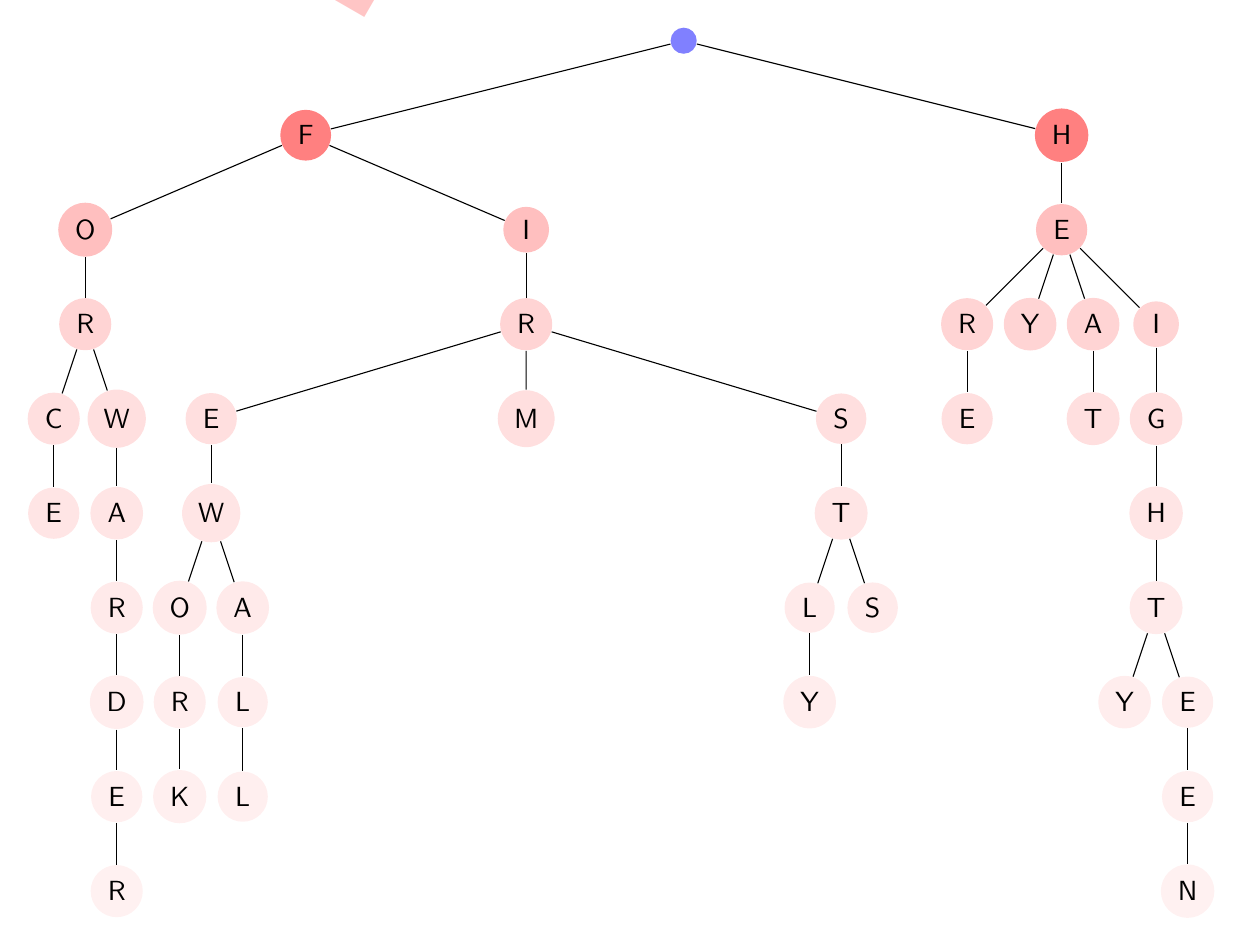
\begin{tikzpicture}[scale=0.8]
\node [circle, fill=blue!50]{}[sibling distance=12cm]
	child{node[circle, fill=red!50.000000]{F}[sibling distance=7cm]
		child{node[circle, fill=red!25.000000]{O}[sibling distance=1cm]
			child{node[circle, fill=red!16.666667]{R}[sibling distance=1cm]
				child{node[circle, fill=red!12.500000]{C}[sibling distance=1cm]
					child{node[circle, fill=red!10.000000]{E}[sibling distance=1cm]
					}
				}
				child{node[circle, fill=red!12.500000]{W}[sibling distance=1cm]
					child{node[circle, fill=red!10.000000]{A}[sibling distance=1cm]
						child{node[circle, fill=red!8.333333]{R}[sibling distance=1cm]
							child{node[circle, fill=red!7.142857]{D}[sibling distance=1cm]
								child{node[circle, fill=red!6.250000]{E}[sibling distance=1cm]
									child{node[circle, fill=red!5.555556]{R}[sibling distance=1cm]
									}
								}
							}
						}
					}
				}
			}
		}
		child{node[circle, fill=red!25.000000]{I}[sibling distance=1cm]
			child{node[circle, fill=red!16.666667]{R}[sibling distance=5cm]
				child{node[circle, fill=red!12.500000]{E}[sibling distance=1cm]
					child{node[circle, fill=red!10.000000]{W}[sibling distance=1cm]
						child{node[circle, fill=red!8.333333]{O}[sibling distance=1cm]
							child{node[circle, fill=red!7.142857]{R}[sibling distance=1cm]
								child{node[circle, fill=red!6.250000]{K}[sibling distance=1cm]
								}
							}
						}
						child{node[circle, fill=red!8.333333]{A}[sibling distance=1cm]
							child{node[circle, fill=red!7.142857]{L}[sibling distance=1cm]
								child{node[circle, fill=red!6.250000]{L}[sibling distance=1cm]
								}
							}
						}
					}
				}
				child{node[circle, fill=red!12.500000]{M}[sibling distance=1cm]
				}
				child{node[circle, fill=red!12.500000]{S}[sibling distance=1cm]
					child{node[circle, fill=red!10.000000]{T}[sibling distance=1cm]
						child{node[circle, fill=red!8.333333]{L}[sibling distance=1cm]
							child{node[circle, fill=red!7.142857]{Y}[sibling distance=1cm]
							}
						}
						child{node[circle, fill=red!8.333333]{S}[sibling distance=1cm]
						}
					}
				}
			}
		}
	}
	child{node[circle, fill=red!50.000000]{H}[sibling distance=1cm]
		child{node[circle, fill=red!25.000000]{E}[sibling distance=1cm]
			child{node[circle, fill=red!16.666667]{R}[sibling distance=1cm]
				child{node[circle, fill=red!12.500000]{E}[sibling distance=1cm]
				}
			}
			child{node[circle, fill=red!16.666667]{Y}[sibling distance=1cm]
			}
			child{node[circle, fill=red!16.666667]{A}[sibling distance=1cm]
				child{node[circle, fill=red!12.500000]{T}[sibling distance=1cm]
				}
			}
			child{node[circle, fill=red!16.666667]{I}[sibling distance=1cm]
				child{node[circle, fill=red!12.500000]{G}[sibling distance=1cm]
					child{node[circle, fill=red!10.000000]{H}[sibling distance=1cm]
						child{node[circle, fill=red!8.333333]{T}[sibling distance=1cm]
							child{node[circle, fill=red!7.142857]{Y}[sibling distance=1cm]
							}
							child{node[circle, fill=red!7.142857]{E}[sibling distance=1cm]
								child{node[circle, fill=red!6.250000]{E}[sibling distance=1cm]
									child{node[circle, fill=red!5.555556]{N}[sibling distance=1cm]
									}
								}
							}
						}
					}
				}
			}
		}
	}
;
\end{tikzpicture}

}

The preceding diagram was created by a parallel program (developed in the appendices) that allows visual trees to be created from a trie. Please note that this is only legible for small trees (beyond that, the branches overlap). This illustration has enabled me to understand all the features implemented and to check that all states are easily correct.

You can see how the tries finds a word visually. This function has been coded to transform \type{trie} into \textit{tikz}. In this way, the word can be retrieved letter by letter by browsing the trie.\\

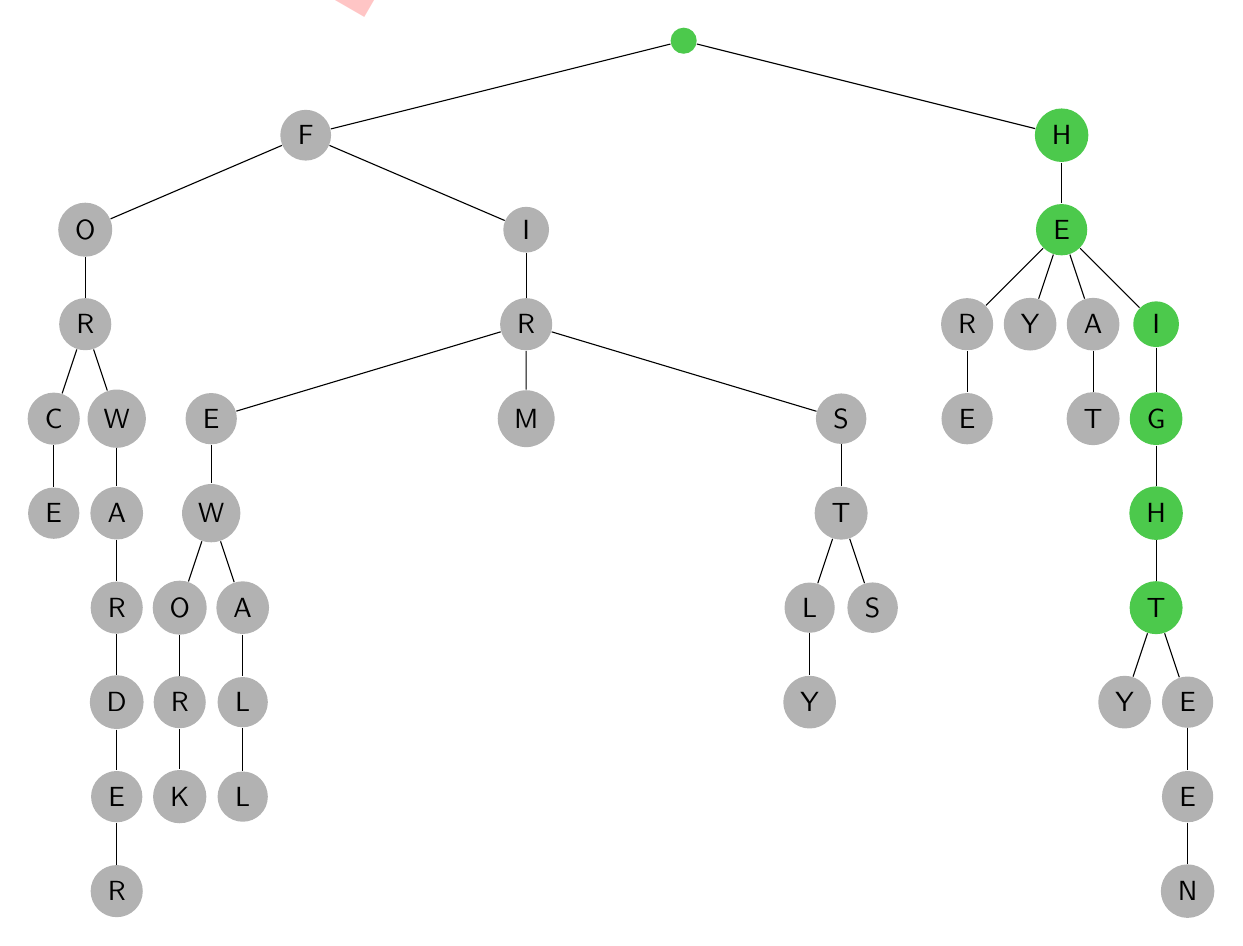
\begin{tikzpicture}[scale=0.8]
\node [circle, fill=green!70!black!70]{}[sibling distance=12cm]
	child{node[circle, fill=black!30]{F}[sibling distance=7cm]
		child{node[circle, fill=black!30]{O}[sibling distance=1cm]
			child{node[circle, fill=black!30]{R}[sibling distance=1cm]
				child{node[circle, fill=black!30]{C}[sibling distance=1cm]
					child{node[circle, fill=black!30]{E}[sibling distance=1cm]
					}
				}
				child{node[circle, fill=black!30]{W}[sibling distance=1cm]
					child{node[circle, fill=black!30]{A}[sibling distance=1cm]
						child{node[circle, fill=black!30]{R}[sibling distance=1cm]
							child{node[circle, fill=black!30]{D}[sibling distance=1cm]
								child{node[circle, fill=black!30]{E}[sibling distance=1cm]
									child{node[circle, fill=black!30]{R}[sibling distance=1cm]
									}
								}
							}
						}
					}
				}
			}
		}
		child{node[circle, fill=black!30]{I}[sibling distance=1cm]
			child{node[circle, fill=black!30]{R}[sibling distance=5cm]
				child{node[circle, fill=black!30]{E}[sibling distance=1cm]
					child{node[circle, fill=black!30]{W}[sibling distance=1cm]
						child{node[circle, fill=black!30]{O}[sibling distance=1cm]
							child{node[circle, fill=black!30]{R}[sibling distance=1cm]
								child{node[circle, fill=black!30]{K}[sibling distance=1cm]
								}
							}
						}
						child{node[circle, fill=black!30]{A}[sibling distance=1cm]
							child{node[circle, fill=black!30]{L}[sibling distance=1cm]
								child{node[circle, fill=black!30]{L}[sibling distance=1cm]
								}
							}
						}
					}
				}
				child{node[circle, fill=black!30]{M}[sibling distance=1cm]
				}
				child{node[circle, fill=black!30]{S}[sibling distance=1cm]
					child{node[circle, fill=black!30]{T}[sibling distance=1cm]
						child{node[circle, fill=black!30]{L}[sibling distance=1cm]
							child{node[circle, fill=black!30]{Y}[sibling distance=1cm]
							}
						}
						child{node[circle, fill=black!30]{S}[sibling distance=1cm]
						}
					}
				}
			}
		}
	}
	child{node[circle, fill=green!70!black!70]{H}[sibling distance=1cm]
		child{node[circle, fill=green!70!black!70]{E}[sibling distance=1cm]
			child{node[circle, fill=black!30]{R}[sibling distance=1cm]
				child{node[circle, fill=black!30]{E}[sibling distance=1cm]
				}
			}
			child{node[circle, fill=black!30]{Y}[sibling distance=1cm]
			}
			child{node[circle, fill=black!30]{A}[sibling distance=1cm]
				child{node[circle, fill=black!30]{T}[sibling distance=1cm]
				}
			}
			child{node[circle, fill=green!70!black!70]{I}[sibling distance=1cm]
				child{node[circle, fill=green!70!black!70]{G}[sibling distance=1cm]
					child{node[circle, fill=green!70!black!70]{H}[sibling distance=1cm]
						child{node[circle, fill=green!70!black!70]{T}[sibling distance=1cm]
							child{node[circle, fill=black!30]{Y}[sibling distance=1cm]
							}
							child{node[circle, fill=black!30]{E}[sibling distance=1cm]
								child{node[circle, fill=black!30]{E}[sibling distance=1cm]
									child{node[circle, fill=black!30]{N}[sibling distance=1cm]
									}
								}
							}
						}
					}
				}
			}
		}
	}
;
\end{tikzpicture}



\subsection{Main counting function}
I've chosen not to restrict the dictionary too much, for example by forcing the deletion of accents, a special case for letters... Indeed, as the \textit{trie} is built from a given dictionary, and the latter is also used for word extraction and validation, all words share the same characters.

\begin{lstlisting}[language=Python, caption=Test all permutations]
def word_game_main_function(self, letters_list: list[str]) -> tuple[int, list[str]]:
    '''Return words built by given letters'''
    counter = 0
    words = []
    for i in range(3, len(letters_list) + 1):
        for permutation in permutations(letters_list, i):
            word = ''.join(permutation)
            if self.search(word):
                counter += 1
                words.append(word)
    return counter, words
\end{lstlisting}

The program line \verb|permutations(letters_list, i)| generates all possible permutations using the lib \verb|permutations| of \verb|itertools| of length $i$. Beware, however, of the complexity of this operation.\\

Let say we have a word $W$ of $m$ letters.
The number of subwords of length k in an m-letter word can be calculated using the combination formula. For a word of m letters, there are C(m, k) subwords of length k, where C(m, k) represents the number of combinations of m elements taken k to k. The formula for C(m, k) is :
$$C(m, k) = \dfrac{m!}{k!(m - k)!}$$
Therefore, the total number of possible subwords in a word of m letters is the sum of the number of subwords of each length:
\begin{equation}
\text{Total number of subwords} = \sum_{k=3}^{m}C(m, k)
\label{eq:number_of_combination}
\end{equation}
Please note that this approach starts counting word from 3 letters and includes the word itself (of length m).
If you need a more specific answer, please provide the length m of the word you have and the more detailed context of what you mean by "subwords".
\begin{figure}[h]
    \centering
    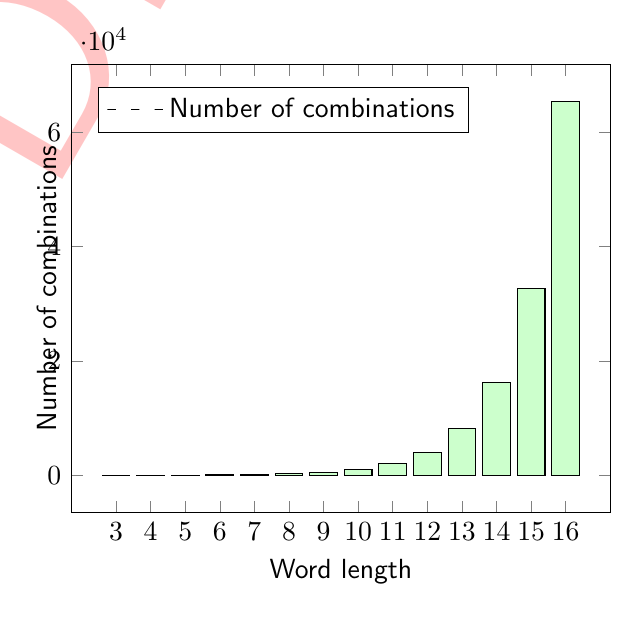
\begin{tikzpicture}
        \begin{axis}[
            xlabel=Word length,
            ylabel=Number of combinations,
            ylabel style={yshift=-10pt},
            xtick=data,
            legend style={at={(0.05,0.95)},anchor=north west}
            ]
        \addplot[ybar, bar width=10pt, fill=green!20]
            coordinates {
                (3, 0)
                (4, 4)
                (5, 15)
                (6, 41)
                (7, 98)
                (8, 218)
                (9, 465)
                (10, 967)
                (11, 1980)
                (12, 4016)
                (13, 8099)
                (14, 16277)
                (15, 32646)
                (16, 65398)
                };
        \legend{Number of combinations} 
        \end{axis}
    \end{tikzpicture}
\end{figure}

As each word generated will pass through the computer, it may be useful to reduce the unit complexity of each test as much as possible. We might consider storing words that are not in the tree in a list (at least their radical) to eradicate all words in the same family. However, this technique requires the creation of a new trie and is therefore unsatisfactory.

\subsection{Interactive function}
\begin{itemize}
    \item To launch the \textit{Interactive} mode, set the \verb|MODE_AUTO| variable to \verb|False|.
    \item You can then set the user input in the function call:
\begin{lstlisting}[language=Python]
results = manual_mode(trie, ['f', 'o', 'r', 'c', 'e'])
\end{lstlisting}
    \item You can then run the program from the command line (don't forget to activate the \verb|venv|):
\begin{lstlisting}
python3 word_challenge.py
\end{lstlisting}
\end{itemize}

\subsection{Automatic execution}
\begin{itemize}
    \item To launch the \textit{Automatic} mode, set the \verb|MODE_AUTO| variable to \verb|True|.
    \item You can then set the number of letters to attempt in the following line:
\begin{lstlisting}[language=Python]
results = automated_mode(trie, 9)
\end{lstlisting}

    \item You can then run the program from the command line (don't forget to activate the \verb|venv|) AND enter a number of words on the command line:
\begin{lstlisting}[language=Bash]
python3 word_challenge.py 100
\end{lstlisting}
\end{itemize}
Program philosophy :
\begin{itemize}
    \item The user enters in CLI a number of words to be tested
    \item After selecting a random word from the dictionary, the program randomly shuffles the letters (displayed as a list) using the \verb|random.shuffle| function.
    \item This list is given to the \verb|word_game_main_function| method, which returns the counter of subwords found in this list of letters.
    \item These counters are then displayed in an tabular in CLI and stored in a \verb|.json| file.
\end{itemize}

\begin{table}[!ht]
    \centering
    \begin{tabular}{|c|c|c|c|}
        \hline
        Iteration & Initial length & CPU time & Word counter \\ \hline
        0 & 8 & 0.020746946334838867 & 72 \\ 
        1 & 10 & 1.9368188381195068 & 150 \\
        2 & 9 & 0.18332123756408691 & 120 \\ 
        3 & 5 & 0.00010991096496582031 & 11 \\ 
        ... & ~ & ~ & ~ \\ 
        49 & 11 & 22.33514976501465 & 721 \\ 
        \hline
        \hline
        AVG: & - & 0.989194917678833 & 71.22 \\ 
        \hline
    \end{tabular}
    \caption{Sample performances}
\end{table}

\subsubsection{Interact with dictionary}
\paragraph{Select random word}
To retrieve random words, you need to select a random line and extract the corresponding word. To do this, we open the file, calculate the total number of lines in the dictionary (with a simple \verb|sum| function), then extract the single line bearing that index (by enumeration). The result is something of the form \verb|future:121844371|. We then extract the word using the following method:
\begin{lstlisting}[language=Python]
word = line.strip().split(':')[0]
\end{lstlisting}
Another method was used with a \textit{regex}: \verb|r'^(?:[a-zA-Z]+)'|

To select a word of a defined length, we use a \type{Trie}. The \type{Trie} can be randomly scanned until a word of the desired length is found for which the last letter has the \verb|is_end_word| attribute. You can also select a word at random until you obtain a word of the desired length. This will take longer, but is relatively negligible compared to the effort required to implement the other method.

The following functions are in the \verb|set_dictionary| file.
\paragraph{Build trie with dictionary words}
In the same way, and as we'll need to do later on, we can build a trie with all the words in the dictionary, to be used later in the word search. We then rely on the methods implemented in the \type{Trie} data structures, such as the \verb|insert_word| method, which we iterate over each word in the dictionary. Here's how it looks:
\begin{lstlisting}[language=Python]
def build_trie(file_path: str) -> Trie:
    '''Get random line from a goven file'''
    dictionary_trie = Trie()

    with open(file_path, 'r') as file:
        for line in file:
            dictionary_trie.insert_word(line.strip().split(':')[0])

    return dictionary_trie
\end{lstlisting}

\paragraph{Get alphabet}
Later (in the Wordle exercise), we'll need to build words from an alphabet. To use the right letters in this step, we need to have the same dictionary we used to check the presence of words in the dictionary. So, when selecting letters, we make sure we have the same letters. In this way, we ensure that we can compare words regardless of the dictionary. In the future, for example, we'll also be able to use non-alphanumeric symbols.\\

We use a \type{set} structure because it's exactly what we want in terms of adding letters. Indeed, a letter is only added to the alphabet if it isn't already in it.\label{set}
The finite alphabet $\Sigma$ is defined dynamically by extracting the set of characters from the set of words in the dictionary:
$$\Sigma = \{\sigma_i\}_{i\in[1, m]},\; m\geqslant 2$$
Let $D$ be the dictionary and $w$ a word in this dictionary, $c$ a letter/character:
$$\Sigma = \bigcup_{w\in D}\{c\in w\}$$

\subsubsection{Performances}
Before testing performance, we need to analyze the data we have to make sure that the dictionary doesn't restrict our analysis. We therefore propose to display the quantity of each word by word size:
\begin{figure}[h]
    \centering
    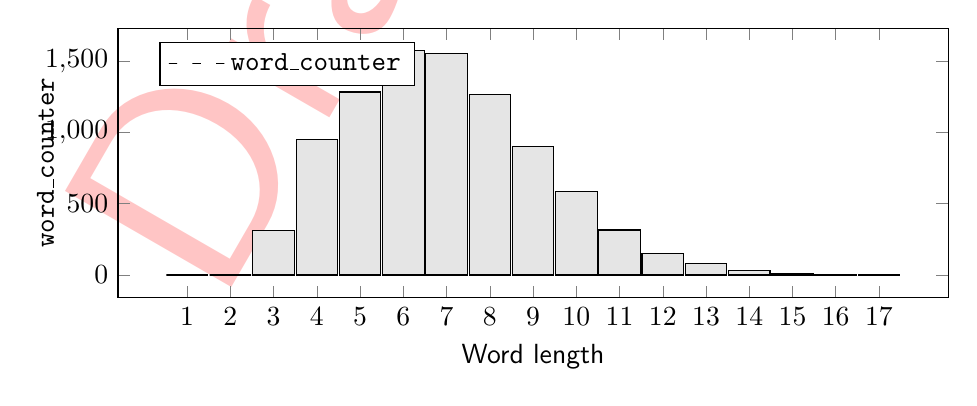
\begin{tikzpicture}
        \begin{axis}[
            xlabel=Word length,
            width=\linewidth,
            height=5cm,
            ylabel=\texttt{word\_counter},
            ylabel style={yshift=-10pt},
            xtick=data,
            legend style={at={(0.05,0.95)},anchor=north west}
            ]
        \addplot[ybar, bar width=15pt, fill=gray!20]
            coordinates {
                (1, 0)
                (2, 0)
                (3, 312)
                (4, 950)
                (5, 1285)
                (6, 1575)
                (7, 1557)
                (8, 1267)
                (9, 904)
                (10, 584)
                (11, 316)
                (12, 153)
                (13, 79)
                (14, 31)
                (15, 11)
                (16, 4)
                (17, 2)
                };
        \legend{ \texttt{word\_counter} } 
        \end{axis}
    \end{tikzpicture}
\end{figure}

To test the performance of this algorithm, we'll be using the automatic mode exclusively. I've chosen to separate the execution and data processing into two parts: retrieve the performance and then analyze it. The first is to extract the performance with the command \verb|python3 word_challenge.py 100|, taking care to set the word length to $0$ to avoid restricting the program with a certain length.\\

You can then run the accompanying program to generate the histograms:
\begin{lstlisting}
python3 additional_algorithms/print_word_challenge_perf.py
\end{lstlisting}
This creates a \verb|.tex| file in the images folder of the documentation folder with the graph in question.\\
\newpage
\begin{figure}[h]
    \centering

    \begin{subfigure}[b]{0.45\textwidth}
        \centering
        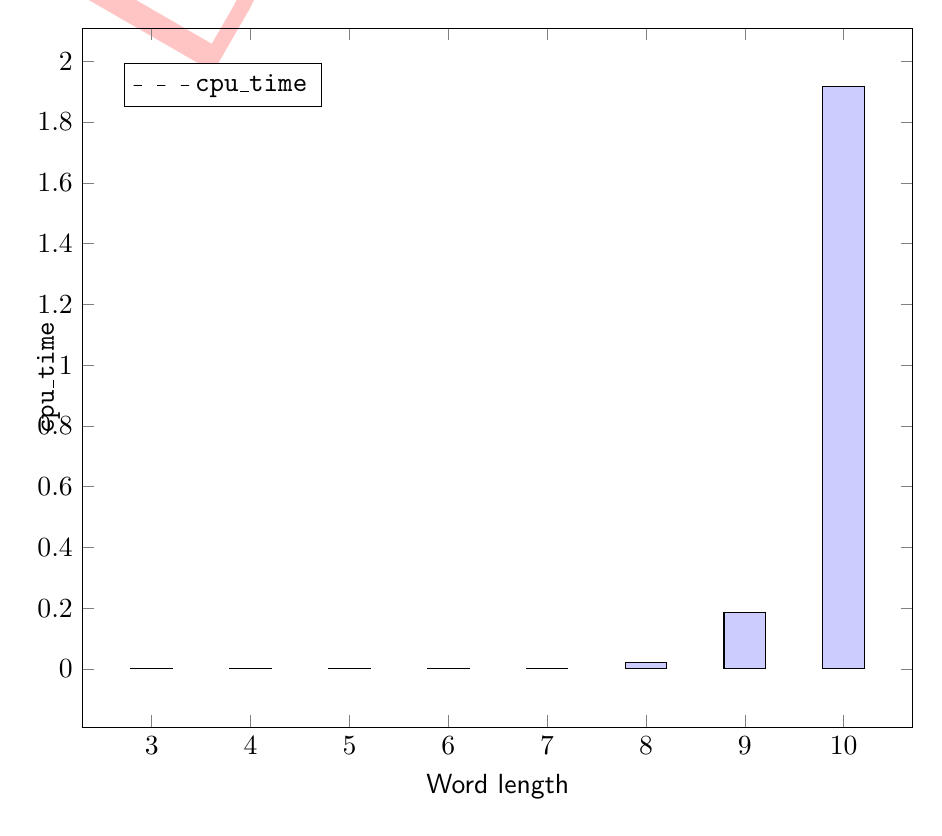
\begin{tikzpicture}
            \begin{axis}[
                xlabel=Word length,
                ylabel=\texttt{cpu\_time},
                ylabel style={yshift=-15pt},
                xtick=data,
                width=\linewidth,
                legend style={at={(0.05,0.95)},anchor=north west},
                ]
            \addplot[ybar, bar width=15pt, fill=blue!20]
                coordinates {
                    (3, 5.6425730387369794e-06)(4, 1.9073486328125e-05)(5, 8.714900297277113e-05)(6, 0.0004047552744547526)(7, 0.0025780797004699707)(8, 0.02060066952424891)(9, 0.18696789308027786)(10, 1.9171473185221355)
                    };
            \legend{ \texttt{cpu\_time} } 
            \end{axis}
        \end{tikzpicture}
    \end{subfigure}
    % \hfill
    \begin{subfigure}[b]{0.45\textwidth}
        \centering
        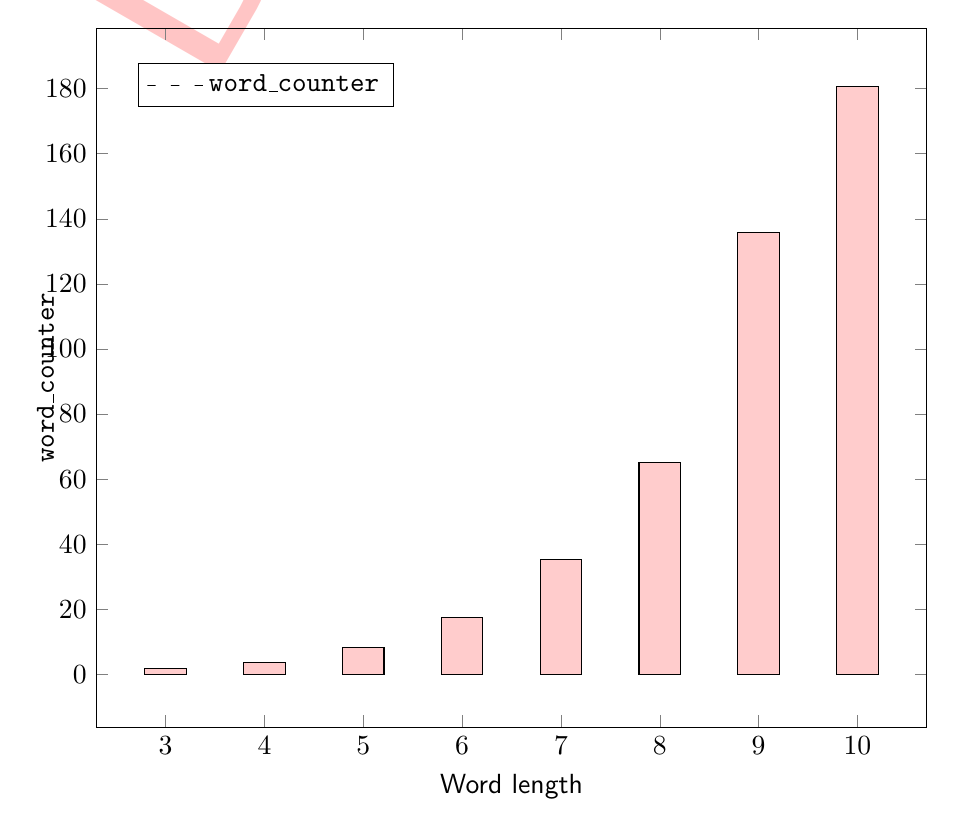
\begin{tikzpicture}
            \begin{axis}[
                xlabel=Word length,
                width=\linewidth,
                ylabel=\texttt{word\_counter},
                ylabel style={yshift=-10pt},
                xtick=data,
                legend style={at={(0.05,0.95)},anchor=north west}
                ]
            \addplot[ybar, bar width=15pt, fill=red!20]
                coordinates {
                    (3, 1.6666666666666667)(4, 3.7)(5, 8.294117647058824)(6, 17.428571428571427)(7, 35.25)(8, 65.23529411764706)(9, 135.9090909090909)(10, 180.66666666666666)
                    };
            \legend{ \texttt{word\_counter} } 
            \end{axis}
        \end{tikzpicture}
    \end{subfigure}
    \caption{Performances testing through process}
\end{figure}
This divergence can be explained by the way words are constructed. While there are more letters available for long words, this creates many more words that don't exist in the dictionary. We could have fun calculating the proportion of valid and invalid words among all the permutations proposed by a set of letters.\\

You'll notice that with 12 or more letters, the program is very, very slow and doesn't converge quickly. Indeed, the equation \ref{eq:number_of_combination} gives for 12 characters : 4017 possible words to test.

\section{Wordle}
\begin{exercise_description}{Wordle}
    In Wordle (\url{https://en.wikipedia.org/wiki/Wordle}) the user can choose to play as \textit{keeper} or as \textit{guesser}. The length $\ell$ of the secret word is defined at the beginning of the game. When playing as \textit{guesser}, the program chooses a secret word of length $\ell$ and for each round the player writes a valid word of length $\ell$ and the computer outputs a string of digits with the following meaning: 0=the corresponding letter does not occur in the secret word, 1=the corresponding letter occurs in the secret word but not at that position, and 2=the corresponding letter occurs at that position. For example, if the secret word were \verb|WORDS| and the current guess were \verb|WHERE|, the program should output \verb|20010|, the \verb|W| was correctly guessed and the \verb|R| is on the secret word, but it is not in the fourth position. The game ends when the secret word is correctly guessed or some \verb|MAX_GUESSES| bound attained. When the player takes the role of the keeper, the computer will make the guesses and the user will give the answers (the strings of 0s, 1s, and 2's).\\

    Finally the program should offer an automatic mode in which the computer plays both as keeper and guesser (without cheating, the guesser function does not have access to the secret word, only its length $\ell$ and the history so far of guesses and answers). For the automatic mode, the human user fixes a length $\ell$ and a (large) number of games to be played. For each game, the keeper chooses a random word of length $\ell$ and a game is played between the keeper and the guesser. At the end, the program outputs the average number of rounds needed by the guesser to guess each secret word and the average CPU time to do it.     
\end{exercise_description}

\subsection*{Execute the programms}
\label{section:notice_wordle}
For all programs, don't forget to activate the \verb|venv|, then run the following command, setting the parameters as follows:
\begin{lstlisting}[language=Python]
python3 wordle_game.py
\end{lstlisting}
\begin{itemize}
    \item To run the interactive guesser program, run the following command:
\begin{lstlisting}[language=Python]
AUTOMATIC_MODE = False
GUESSER = True
KEEPER = False
\end{lstlisting}
    \item To run the keeper interactive program, run the following command:
\begin{lstlisting}[language=Python]
AUTOMATIC_MODE = False
GUESSER = False
KEEPER = True
\end{lstlisting}
    \item To run the automatic program for 1 puzzle only
\begin{lstlisting}[language=Python]
AUTOMATIC_MODE = True
AUTOMATIC_MODE_GENERATOR = False
\end{lstlisting}
    \item To run the automatic program for 200 puzzles for the first 3 word lengths $\ell\in\{3, 4, 5\}$.
\begin{lstlisting}[language=Python]
AUTOMATIC_MODE = True
AUTOMATIC_MODE_GENERATOR = True
\end{lstlisting}
\end{itemize}

\subsection{Guesser mode}
\paragraph{Principle}
The principle of the game is defined in the instructions. I'll just explain the implementation and the choice of functions. Here's how the program works. The complete program can be found in the file \verb|wordle_guesser.py|.
\begin{enumerate}
    \item The program selects a random word from the provided dictionary
    \item It then asks the user (or the keeper program in the following) to suggest a guess
    \item It compares letter by letter whether the letter at this index is identical to the one at the same index in the secret.
    \item If it is, then the status is set to 2 and stored in a temporary list
    \item If not, it checks whether the proposed letter is present in the secret (and returns 1 or 0 depending on its presence)
    \item The program finally returns the concatenated scores to the user.
    \item This program continues until the user is successful or has exceeded the number of possible attempts. 
\end{enumerate}
\textcolor{red}{Please note: please note that in the following, the program names correspond to what the user has to do. This is due to an ambiguous reading of the statement. The function of the program is therefore the opposite of what its name suggests. The guesser function doesn't guess, but lets the user guess by guiding him/her, while the function tries to guess while the user keeps the secret and gives the letter scores.}.
\paragraph{Human interaction}
I separate the reception from the human/machine interaction in a separate function so that I can use python's \verb|input| function, then parse the result for inclusion in the program later.\\

\paragraph{Scores in array or string ?}
\begin{itemize}
    \item Working with numeric strings is not a simple matter for analysis. You then have to parse it to extract the scores in integer form. This is the subject of an intermediate function. It's because we're asked to work with numeric strings like \verb|112001| that we do it. It's only simpler in the case of human/machine interaction.
    \item Whatever happens, within programs, scores will be used via lists, by the following translation for example:
\begin{lstlisting}[language=Python]
result_array = [0 for _ in range(word_length)]
\end{lstlisting}
Then the reverse translation (transformation of the list into a character string):
\begin{lstlisting}[language=Python]
''.join(map(str, result_array))
\end{lstlisting}
\end{itemize}

\subsection{Keeper mode}
This was the most complex part of the game to model, in order to make it as quick as possible. Indeed, a naive approach to this exercise would be to select random letters to compose a word, submit it to the test to obtain the evaluation (in 0, 1 and 2) then test another and so on. As the tests progressed, I developed new features to avoid unnecessary iterations, as we'll see in this section.

\subsection{Data structures used}
Each guess is treated as a separate guess, linked to the previous information received by the guesser. In this way, we can capitalize - as a normal player would - on previous guesses. To do this, I've chosen to develop a new data structure grouping together the information useful for constructing each guess (grouping together the letters to be tried first, those that will lead to uselessness...).

\paragraph{\type{WordLetter}} Think of the game as a series of guesses to position strategic letters. We can therefore create a resolution strategy to reduce the number of attempts.
\begin{itemize}
    \item For example, we can store all the letters that have already been unsuccessfully tested so as not to try them again, as this would lead to useless attempts. Beware, however: by removing this possibility, we also remove a large number of valid words that would have enabled us to detect potential new letters.
    \item I'd also suggest implementing a boolean in the \verb|blocked_letter| field to indicate whether the letter has been found or not ($=2$). In this case, there's no need to generate new letters.
\end{itemize}

\begin{figure}[h]
    \centering
    \begin{tikzpicture}
        \node[draw, rounded corners=2mm, inner sep = 0.2cm, fill=orange!0] { 
        \begin{tikzpicture} 
            \node[inner sep = 1mm] (title) { \Large{\bfseries WordLetter }}; 
            % \draw (title.south west) -- (title.south east);
            \node[at=(title.south), anchor=north, inner sep=3mm, align=left, fill=green!30!black!10, yshift=-0.2cm] (attributes) {
                \begin{minipage}{60mm}
                    \textbf{Attributes}\\
                    \small{0}: \verb|index|\\
\small{1}: \verb|past_letters|\\
\small{2}: \verb|score|\\
\small{3}: \verb|blocked_letter|\\
\small{4}: \verb|current_letter|
                \end{minipage} 
                };
            % \draw (attributes.north west) -- (attributes.north east);
            \node[at=(attributes.south), anchor=north, inner sep=3mm, align=left, fill=blue!10, yshift=-0.2cm] (methods) {
                \begin{minipage}{60mm}
                    \textbf{Methods}\\
                    \small{0}: \verb|add_letter_guess|\\
\small{1}: \verb|add_past_letter|\\
\small{2}: \verb|block_letter|\\
\small{3}: \verb|is_past_letter|\\
\small{4}: \verb|update_score|
                \end{minipage} 
                };
            % \draw (methods.north west) -- (methods.north east);
        \end{tikzpicture}
        }; 
    \end{tikzpicture}
    \caption{Class description - WordLetter }
    \label{class:WordLetter}
\end{figure}
\begin{itemize}
    \item This object is also provided with methods for performing the previous functions, such as adding a new letter to the list of letters already tested.
\end{itemize}

In conclusion, letters become objects with properties that make them intelligent, rather than just random letters in a word. Part of the logic of the game is thus transferred to the logic of the letters.


\paragraph{\type{Guess}} The data structure aims to model the reasoning one might have when playing Wordle as a human. Words are made up of ordered letters that give rise to trial and error.
\begin{itemize}
    \item We choose to model the guess as a sequence of $m$ letters ordered by their \verb|index|. Each letter is initialized at the start of the game and then fed by other letters. The guess is also given an alphabet so that it knows which finite sequence of letters to draw from to make up the words.
    \item Letters that have already been tested and failed ($=0$) are stored in a black list (type: \type{set}) so that they are not tested again, regardless of the letter \verb|bad_letters|. Next, letters that have been tested but incorrectly positioned($=1$) are stored in a \type{set} \verb|incorrect_position_letters|.
\end{itemize}
\begin{figure}[h]
    \centering
    \begin{tikzpicture}
        \node[draw, rounded corners=2mm, inner sep = 0.2cm, fill=orange!0] { 
        \begin{tikzpicture} 
            \node[inner sep = 1mm] (title) { \Large{\bfseries Guess }}; 
            % \draw (title.south west) -- (title.south east);
            \node[at=(title.south), anchor=north, inner sep=3mm, align=left, fill=green!30!black!10, yshift=-0.2cm] (attributes) {
                \begin{minipage}{60mm}
                    \textbf{Attributes}\\
                    \small{0}: \verb|letters|\\
\small{1}: \verb|length|\\
\small{2}: \verb|alphabet|\\
\small{3}: \verb|incorrect_position_letters|\\
\small{4}: \verb|bad_letters|\\
\small{5}: \verb|remaining_letters|\\
\small{6}: \verb|dictionary_trie|
                \end{minipage} 
                };
            % \draw (attributes.north west) -- (attributes.north east);
            \node[at=(attributes.south), anchor=north, inner sep=3mm, align=left, fill=blue!10, yshift=-0.2cm] (methods) {
                \begin{minipage}{60mm}
                    \textbf{Methods}\\
                    \small{0}: \verb|actualize_letter|\\
\small{1}: \verb|actualize_letters_informations|\\
\small{2}: \verb|display_word|\\
\small{3}: \verb|extract_random_letter|\\
\small{4}: \verb|generate_new_letters|\\
\small{5}: \verb|is_valid_word|\\
\small{6}: \verb|new_guess|
                \end{minipage} 
                };
            % \draw (methods.north west) -- (methods.north east);
        \end{tikzpicture}
        }; 
    \end{tikzpicture}
    \caption{Class description - Guess }
    \label{class:Guess}
\end{figure}

\textbf{Methods}
\begin{itemize}
    \setcounter{enumi}{-1}
    \item \verb|actualize_letter|: test a new letter for a given index
    \item \verb|actualize_letters_informations|: updates the score of each letter before guessing.
    \item \verb|display_word|: Displays the word broken down into a simple \type{WordLetter}.
\end{itemize}

\paragraph{\type{set}}
As mentioned in the \ref{set} paragraph, we're using a set for "forbidden" letters and letters to be positioned in the word, because we're using the \verb|set.add()| property, which allows us to add information only if it's not already entered.

\paragraph{\type{Trie}}
To look up the words and check their existence in the dictionary, we rely on what was programmed in the first part of this assignment. We index all the words in the dictionary into a trie using the \verb|build_trie| function in the \verb|additional_algorithms| folder. Once all the words have been entered in the trie, we can use the previous coded method to check the word's existence in the trie \verb|trie.search(word: str)|.
This will optimize the word search.


\subsection{Automatic mode}
\subsubsection{Different modes}
Two automatic solving modes have been developed, the second of which builds on the first. First, it is important to program the automatic version, which solves a puzzle imposed by the guesser mode. Then, we can try to scale this resolution, which is why we developed the second program.

\paragraph{Classic automatic mode}
This program aims to interface both the \textit{guesser} and the \textit{keeper}. The guesser program responds with the string containing the scores, which is then used to generate a new word, and so on.
\begin{lstlisting}[language=Python]
def guesser_automatic_mode(word_length: int = SECRET_LENGTH,
                            dictionary_path: str = DICTIONARY_PATH,
                            max_attempts: int = MAX_GUESSES
                          ) -> None:

    # Initialisation section : trie, alphabet, secret
    secret = ''
    trie = build_trie(dictionary_path)
    alphabet = set_alphabet(dictionary_path)

    # Define secret (generated)
    while len(secret) != word_length:
        secret = extract_informations(get_random_line(dictionary_path))

    # Set puzzle
    result_array = [0 for _ in range(word_length)]
    attempts = 0
    guess = Guess(word_length, trie, alphabet)

    # Solve puzzle
    while not all(num == 2 for num in result_array) and attempts < max_attempts:
        guess.new_guess([int(score) for score in result_array])
        new_guess = guess.display_word()
        result_array = check_guess(new_guess, secret)

        attempts += 1

    return {
    'solved': all(num == 2 for num in result_array),
    'attempts': attempts,
    'max_attempts': max_attempts,
    'size': word_length
    }

\end{lstlisting}

\paragraph{Generate data to analyse}
For each desired word length (from 3 to 5 in this example), 200 puzzle resolutions are generated by the keeper. This result is then stored in a json file and analyzed with the program \verb|wordle_performance| in the folder \verb|additional_algorithms|. This generates the coordinates of the curves in the performance section. 
The advantage of this solution is that we can extract a lot of data and process it as we want. This is particularly useful to plot the two indicators we need: CPU time and the number of attempts required to find the word.


\subsubsection{Performances}
Pay attention to one point in particular. In this exercise, I chose to focus performance on the minimum number of trials. It might also have been possible to measure CPU time by running more trials.
\paragraph{How many attempts to solve the puzzle?}
We can see from the graph above that the trend in the number of trials to solve the puzzles decreases with increasing word length. This can be explained as follows:
\begin{itemize}
    \item More letters in a word = more letter attempts on each try
    \item So more letters marked as forbidden
    \item These letters are therefore no longer used, making way for new letters that might match (randomly generated letters).
    \item Similarly, by testing more letters, we have more information on the letters with score 1.
\end{itemize}
\begin{figure}[h]
    \centering
    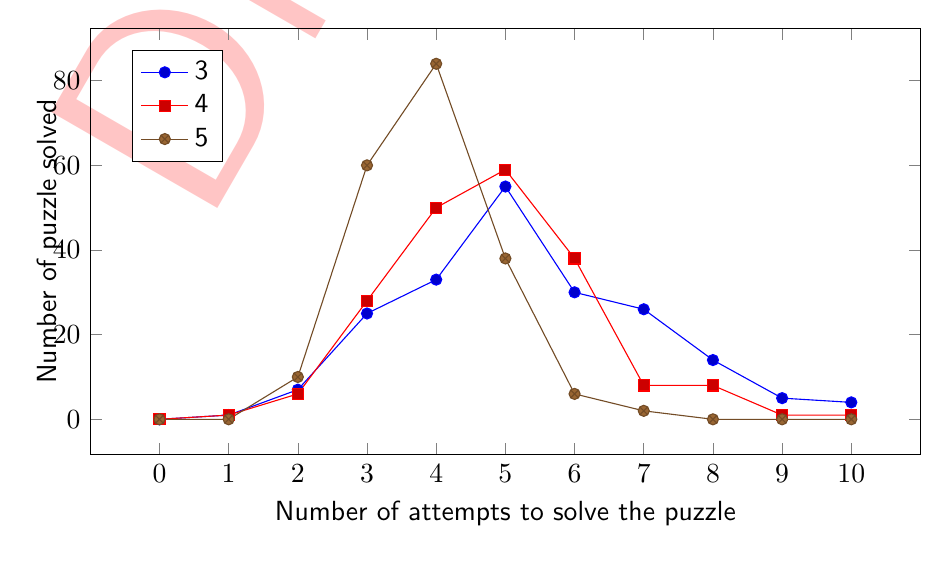
\begin{tikzpicture}
        \begin{axis}[
            xlabel=Number of attempts to solve the puzzle,
            width=\linewidth,
            height=7cm,
            ylabel=Number of puzzle solved,
            ylabel style={yshift=-10pt},
            xtick=data,
            legend style={at={(0.05,0.95)},anchor=north west}
            ]
        \addplot
            coordinates {
                (0, 0)
                (1, 1)
                (2, 7)
                (3, 25)
                (4, 33)
                (5, 55)
                (6, 30)
                (7, 26)
                (8, 14)
                (9, 5)
                (10, 4)
                };
        \addplot
            coordinates {
                (0, 0)
                (1, 1)
                (2, 6)
                (3, 28)
                (4, 50)
                (5, 59)
                (6, 38)
                (7, 8)
                (8, 8)
                (9, 1)
                (10, 1)
                };
            \addplot
            coordinates {
                (0, 0)
                (1, 0)
                (2, 10)
                (3, 60)
                (4, 84)
                (5, 38)
                (6, 6)
                (7, 2)
                (8, 0)
                (9, 0)
                (10, 0)
                };
                       
        \legend{3, 4, 5} 
        \end{axis}
    \end{tikzpicture}
    \caption{Automatic guesser performances measures}
\end{figure}
On average, the program generates the answer to all challenges in less than 5 moves. This performance is achieved at the cost of computation time, which is relatively long for large words.

\paragraph{How much CPU time needed to solve the puzzle?}
We can also ask, as previously mentioned, how much CPU time this resolution represents. This is simply measured by timing the entire resolution part. Since the guesser part is negligible (as it is only constant in time), this almost totally reflects the CPU time dedicated to the keeper. With the following command, you can plot the CPU time graphs for keeper performance (take care to set the program to automatic mode, instructions here: \ref{section:notice_wordle})

\begin{lstlisting}[language=Bash]
python3 wordle_game.py && python3 additional_algorithms/wordle_performance.py
\end{lstlisting}
It is also possible to modify the length of the words tested to obtain better performance, but this would require a calculation over several hours.
\begin{figure}[h]
    \centering
    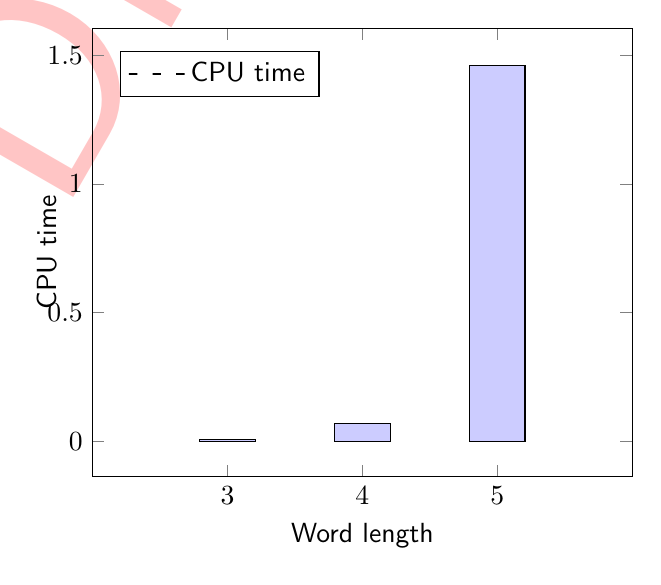
\begin{tikzpicture}
        \begin{axis}[
            xlabel=Word length,
            % width=\linewidth,
            % height=5cm,
            ylabel=CPU time,
            ylabel style={yshift=-10pt},
            xtick=data,
            xmin=2,
            xmax=6,
            legend style={at={(0.05,0.95)},anchor=north west}
            ]
        \addplot[ybar, bar width=20pt, fill=blue!20]
            coordinates {
                (3, 0.00882602334022522)
                (4, 0.06812063932418823)
                (5, 1.4601097178459168)
                };
        \legend{CPU time} 
        \end{axis}
    \end{tikzpicture}
\end{figure}


\section{Appendices}
\subsection{Personal feedback from this exercise}
This exercise was a real learning experience in many respects:
\begin{itemize}
    \item Complex project programming
    \item Technical report writing
    \item Clean coding and good development practices
\end{itemize}

\subsection{Interfacing \textit{tikz} and programs}
\subsubsection{Produce dynamic tries with tikz}
As used in the first sections, we can choose to create a python program that dynamically creates trees in tikz. This allows us to visually represent what's happening in a sort, and thus to adjust parameters, arguments, methods and so on. However, this is only possible for small trees.

\subsubsection{Draw class sumaries}
As used in the first sections, we can choose to create a python program that dynamically creates trees in tikz. This allows us to visually represent what's happening in a trie, and thus to adjust parameters, arguments, methods and so on. However, this is only possible for small trees.




\newpage
\listoffigures
\lstlistoflistings
\listoftables
\end{document}






\begin{figure}[h]
    \centering
    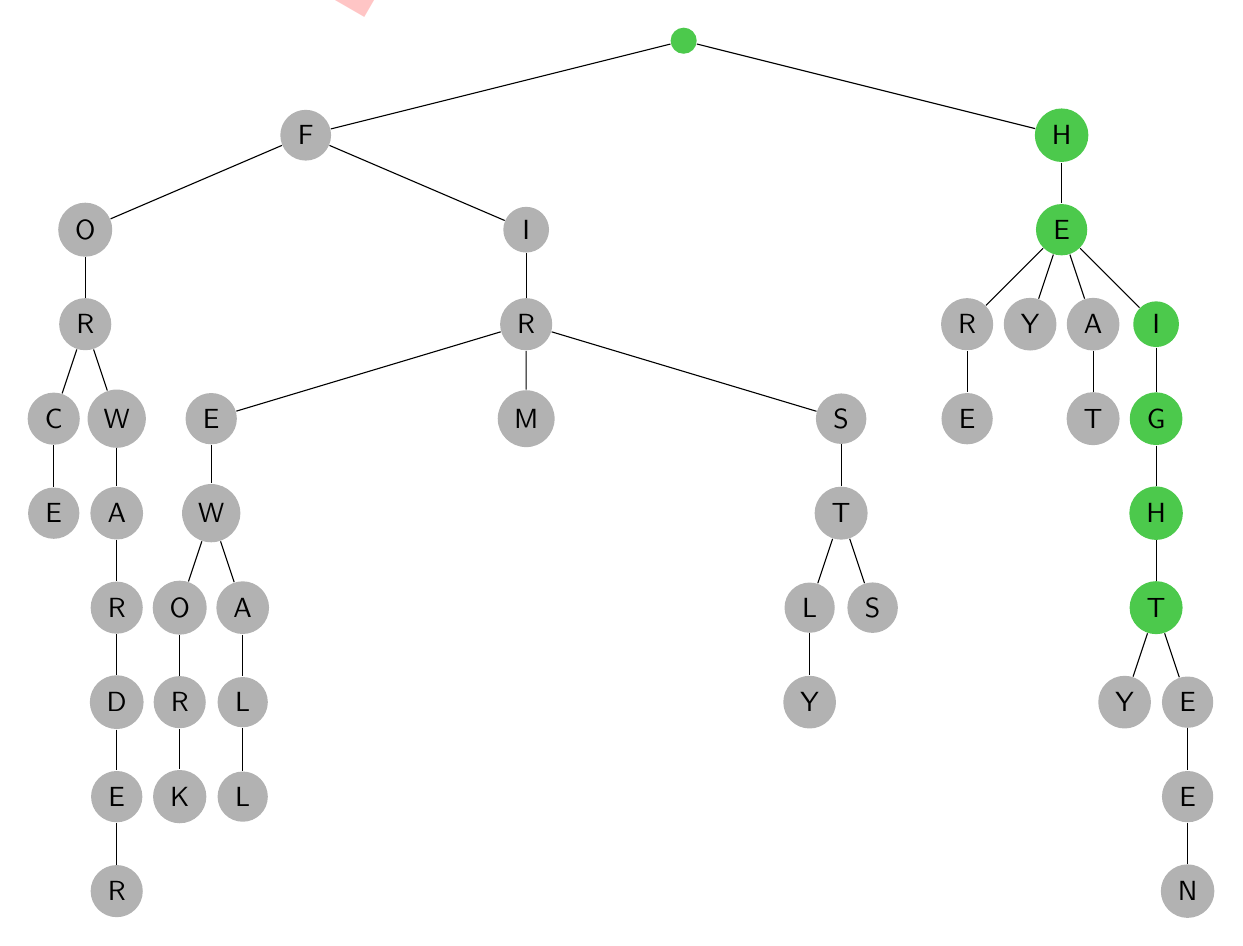
\begin{tikzpicture}[scale=0.8]
\node [circle, fill=green!70!black!70]{}[sibling distance=12cm]
	child{node[circle, fill=black!30]{F}[sibling distance=7cm]
		child{node[circle, fill=black!30]{O}[sibling distance=1cm]
			child{node[circle, fill=black!30]{R}[sibling distance=1cm]
				child{node[circle, fill=black!30]{C}[sibling distance=1cm]
					child{node[circle, fill=black!30]{E}[sibling distance=1cm]
					}
				}
				child{node[circle, fill=black!30]{W}[sibling distance=1cm]
					child{node[circle, fill=black!30]{A}[sibling distance=1cm]
						child{node[circle, fill=black!30]{R}[sibling distance=1cm]
							child{node[circle, fill=black!30]{D}[sibling distance=1cm]
								child{node[circle, fill=black!30]{E}[sibling distance=1cm]
									child{node[circle, fill=black!30]{R}[sibling distance=1cm]
									}
								}
							}
						}
					}
				}
			}
		}
		child{node[circle, fill=black!30]{I}[sibling distance=1cm]
			child{node[circle, fill=black!30]{R}[sibling distance=5cm]
				child{node[circle, fill=black!30]{E}[sibling distance=1cm]
					child{node[circle, fill=black!30]{W}[sibling distance=1cm]
						child{node[circle, fill=black!30]{O}[sibling distance=1cm]
							child{node[circle, fill=black!30]{R}[sibling distance=1cm]
								child{node[circle, fill=black!30]{K}[sibling distance=1cm]
								}
							}
						}
						child{node[circle, fill=black!30]{A}[sibling distance=1cm]
							child{node[circle, fill=black!30]{L}[sibling distance=1cm]
								child{node[circle, fill=black!30]{L}[sibling distance=1cm]
								}
							}
						}
					}
				}
				child{node[circle, fill=black!30]{M}[sibling distance=1cm]
				}
				child{node[circle, fill=black!30]{S}[sibling distance=1cm]
					child{node[circle, fill=black!30]{T}[sibling distance=1cm]
						child{node[circle, fill=black!30]{L}[sibling distance=1cm]
							child{node[circle, fill=black!30]{Y}[sibling distance=1cm]
							}
						}
						child{node[circle, fill=black!30]{S}[sibling distance=1cm]
						}
					}
				}
			}
		}
	}
	child{node[circle, fill=green!70!black!70]{H}[sibling distance=1cm]
		child{node[circle, fill=green!70!black!70]{E}[sibling distance=1cm]
			child{node[circle, fill=black!30]{R}[sibling distance=1cm]
				child{node[circle, fill=black!30]{E}[sibling distance=1cm]
				}
			}
			child{node[circle, fill=black!30]{Y}[sibling distance=1cm]
			}
			child{node[circle, fill=black!30]{A}[sibling distance=1cm]
				child{node[circle, fill=black!30]{T}[sibling distance=1cm]
				}
			}
			child{node[circle, fill=green!70!black!70]{I}[sibling distance=1cm]
				child{node[circle, fill=green!70!black!70]{G}[sibling distance=1cm]
					child{node[circle, fill=green!70!black!70]{H}[sibling distance=1cm]
						child{node[circle, fill=green!70!black!70]{T}[sibling distance=1cm]
							child{node[circle, fill=black!30]{Y}[sibling distance=1cm]
							}
							child{node[circle, fill=black!30]{E}[sibling distance=1cm]
								child{node[circle, fill=black!30]{E}[sibling distance=1cm]
									child{node[circle, fill=black!30]{N}[sibling distance=1cm]
									}
								}
							}
						}
					}
				}
			}
		}
	}
;
\end{tikzpicture}


    \caption{Search path}
    \label{fig:search_path_pgm}
\end{figure}

\begin{figure}[h]
    \centering
    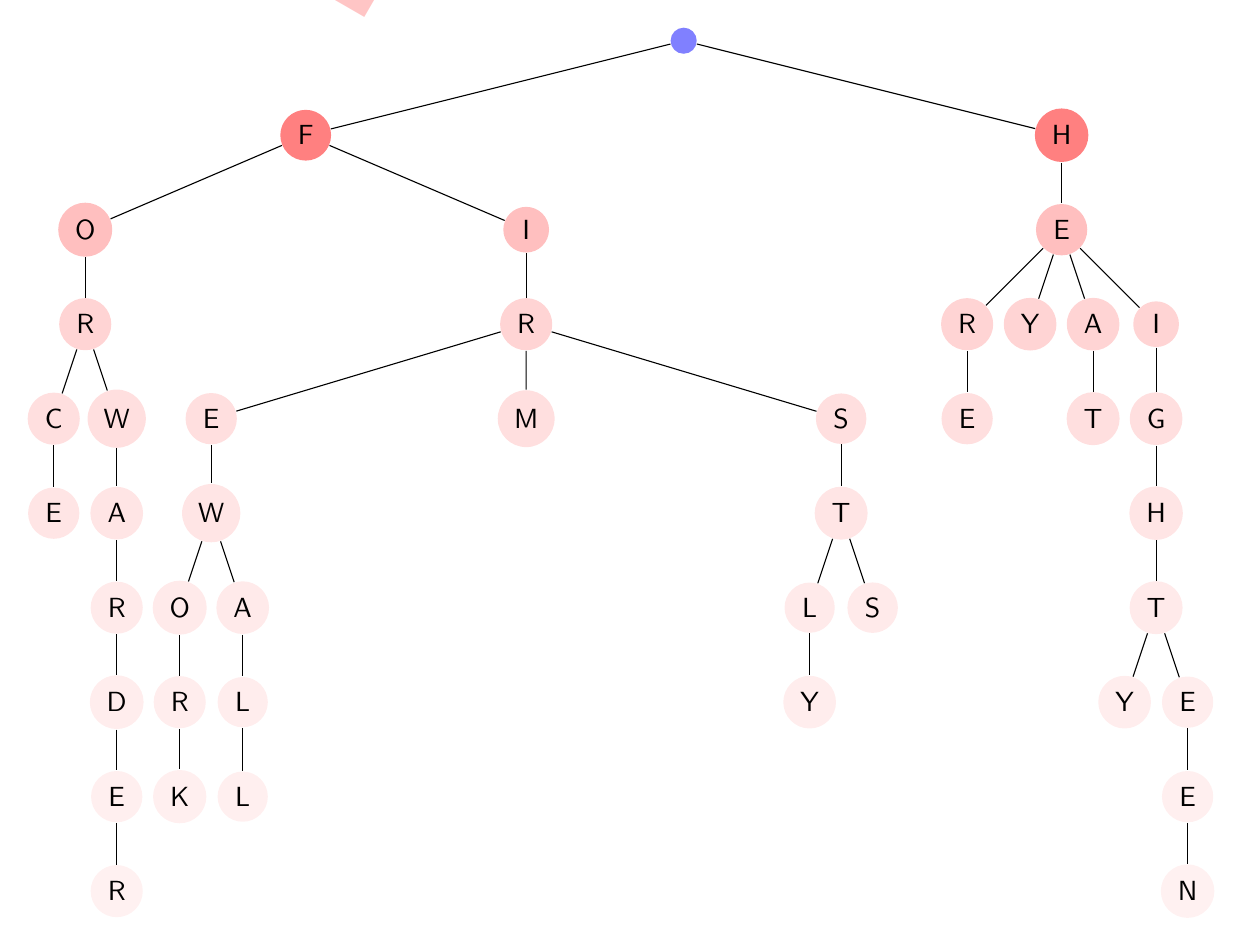
\begin{tikzpicture}[scale=0.8]
\node [circle, fill=blue!50]{}[sibling distance=12cm]
	child{node[circle, fill=red!50.000000]{F}[sibling distance=7cm]
		child{node[circle, fill=red!25.000000]{O}[sibling distance=1cm]
			child{node[circle, fill=red!16.666667]{R}[sibling distance=1cm]
				child{node[circle, fill=red!12.500000]{C}[sibling distance=1cm]
					child{node[circle, fill=red!10.000000]{E}[sibling distance=1cm]
					}
				}
				child{node[circle, fill=red!12.500000]{W}[sibling distance=1cm]
					child{node[circle, fill=red!10.000000]{A}[sibling distance=1cm]
						child{node[circle, fill=red!8.333333]{R}[sibling distance=1cm]
							child{node[circle, fill=red!7.142857]{D}[sibling distance=1cm]
								child{node[circle, fill=red!6.250000]{E}[sibling distance=1cm]
									child{node[circle, fill=red!5.555556]{R}[sibling distance=1cm]
									}
								}
							}
						}
					}
				}
			}
		}
		child{node[circle, fill=red!25.000000]{I}[sibling distance=1cm]
			child{node[circle, fill=red!16.666667]{R}[sibling distance=5cm]
				child{node[circle, fill=red!12.500000]{E}[sibling distance=1cm]
					child{node[circle, fill=red!10.000000]{W}[sibling distance=1cm]
						child{node[circle, fill=red!8.333333]{O}[sibling distance=1cm]
							child{node[circle, fill=red!7.142857]{R}[sibling distance=1cm]
								child{node[circle, fill=red!6.250000]{K}[sibling distance=1cm]
								}
							}
						}
						child{node[circle, fill=red!8.333333]{A}[sibling distance=1cm]
							child{node[circle, fill=red!7.142857]{L}[sibling distance=1cm]
								child{node[circle, fill=red!6.250000]{L}[sibling distance=1cm]
								}
							}
						}
					}
				}
				child{node[circle, fill=red!12.500000]{M}[sibling distance=1cm]
				}
				child{node[circle, fill=red!12.500000]{S}[sibling distance=1cm]
					child{node[circle, fill=red!10.000000]{T}[sibling distance=1cm]
						child{node[circle, fill=red!8.333333]{L}[sibling distance=1cm]
							child{node[circle, fill=red!7.142857]{Y}[sibling distance=1cm]
							}
						}
						child{node[circle, fill=red!8.333333]{S}[sibling distance=1cm]
						}
					}
				}
			}
		}
	}
	child{node[circle, fill=red!50.000000]{H}[sibling distance=1cm]
		child{node[circle, fill=red!25.000000]{E}[sibling distance=1cm]
			child{node[circle, fill=red!16.666667]{R}[sibling distance=1cm]
				child{node[circle, fill=red!12.500000]{E}[sibling distance=1cm]
				}
			}
			child{node[circle, fill=red!16.666667]{Y}[sibling distance=1cm]
			}
			child{node[circle, fill=red!16.666667]{A}[sibling distance=1cm]
				child{node[circle, fill=red!12.500000]{T}[sibling distance=1cm]
				}
			}
			child{node[circle, fill=red!16.666667]{I}[sibling distance=1cm]
				child{node[circle, fill=red!12.500000]{G}[sibling distance=1cm]
					child{node[circle, fill=red!10.000000]{H}[sibling distance=1cm]
						child{node[circle, fill=red!8.333333]{T}[sibling distance=1cm]
							child{node[circle, fill=red!7.142857]{Y}[sibling distance=1cm]
							}
							child{node[circle, fill=red!7.142857]{E}[sibling distance=1cm]
								child{node[circle, fill=red!6.250000]{E}[sibling distance=1cm]
									child{node[circle, fill=red!5.555556]{N}[sibling distance=1cm]
									}
								}
							}
						}
					}
				}
			}
		}
	}
;
\end{tikzpicture}


    \caption{Draw trie}
    \label{fig:draw_pgm}
\end{figure}



\section{Data structure}
\subsection{Tries implementation}


\section{Performances}
\begin{summary}
    Essai
\end{summary}


\section{Complexity and time preduction}


\begin{figure}
    \centering
    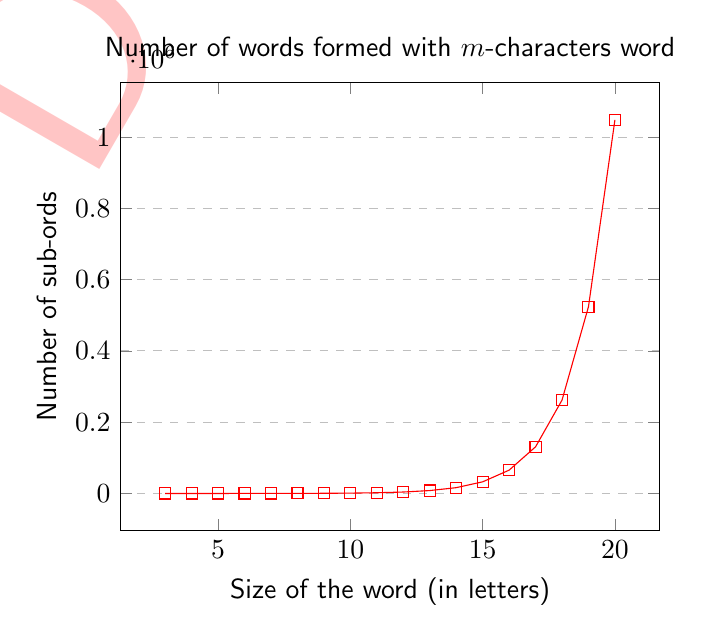
\begin{tikzpicture}
\begin{axis}[
    title={Number of words formed with $m$-characters word},
    xlabel={Size of the word (in letters)},
    ylabel={Number of sub-ords},
    % xmin=0, xmax=100,
    % ymin=0, ymax=120,
    % xtick={0,20,40,60,80,100},
    % ytick={0,20,40,60,80,100,120},
    legend pos=north west,
    ymajorgrids=true,
    grid style=dashed,
]

\addplot[
    color=red,
    mark=square,
    ]
    coordinates {
        (3, 0)
        (4, 4)
        (5, 15)
        (6, 41)
        (7, 98)
        (8, 218)
        (9, 465)
        (10, 967)
        (11, 1980)
        (12, 4016)
        (13, 8099)
        (14, 16277)
        (15, 32646)
        (16, 65398)
        (17, 130917)
        (18, 261971)
        (19, 524096)
        (20, 1048364)
    };
    
\end{axis}
\end{tikzpicture}

    \caption{A PGF histogram from \texttt{matplotlib}.}
\end{figure}

As a consequence, we have to find a way to decrease the number of 

\section{Ideas}
Change the programmation philosophy to:
\begin{itemize}
    \item Définition des fonctions de jeu par récurrence: appel de la fonction avec comme paramètres
        \begin{itemize}
            \item Mot à deviner (secret)
            \item Mot choisi par l'utilisateur
            \item Résultat (en terme de 0, 1, 2)
            \item Numéro de l'essais 
        \end{itemize}
        Cela permettra de faire appel aux fonctions par récurrence et de mutualiser les programmes de \textit{guesser} et de \textit{keeper}
    \item Passer en programmation par objet avec un objet pour :
        \begin{itemize}
            \item guesser
            \item keeper
            \item guess
            \item secret
            \item tentative
        \end{itemize}
\end{itemize}

\section{Best practices}
\begin{itemize}
    \item Description des fonctions avec docstring
    \item Ajout des typages pour les fonctions (aide à l'IDE)
    \item Mise en commun des fonctions identiques (factorisation)
    \item Tentative d'optimisation
\end{itemize}



\section{Objects}
\begin{figure}[h]
    \centering
    \begin{tikzpicture}
        \node[draw, rounded corners=2mm, inner sep = 0.2cm, fill=orange!0] { 
        \begin{tikzpicture} 
            \node[inner sep = 1mm] (title) { \Large{\bfseries Guess }}; 
            % \draw (title.south west) -- (title.south east);
            \node[at=(title.south), anchor=north, inner sep=3mm, align=left, fill=green!30!black!10, yshift=-0.2cm] (attributes) {
                \begin{minipage}{60mm}
                    \textbf{Attributes}\\
                    \small{0}: \verb|letters|\\
\small{1}: \verb|length|\\
\small{2}: \verb|alphabet|\\
\small{3}: \verb|incorrect_position_letters|\\
\small{4}: \verb|bad_letters|\\
\small{5}: \verb|remaining_letters|\\
\small{6}: \verb|dictionary_trie|
                \end{minipage} 
                };
            % \draw (attributes.north west) -- (attributes.north east);
            \node[at=(attributes.south), anchor=north, inner sep=3mm, align=left, fill=blue!10, yshift=-0.2cm] (methods) {
                \begin{minipage}{60mm}
                    \textbf{Methods}\\
                    \small{0}: \verb|actualize_letter|\\
\small{1}: \verb|actualize_letters_informations|\\
\small{2}: \verb|display_word|\\
\small{3}: \verb|extract_random_letter|\\
\small{4}: \verb|generate_new_letters|\\
\small{5}: \verb|is_valid_word|\\
\small{6}: \verb|new_guess|
                \end{minipage} 
                };
            % \draw (methods.north west) -- (methods.north east);
        \end{tikzpicture}
        }; 
    \end{tikzpicture}
    \caption{Class description - Guess }
    \label{class:Guess}
\end{figure}
\begin{figure}[h]
    \centering
    \begin{tikzpicture}
        \node[draw, rounded corners=2mm, inner sep = 0.2cm, fill=orange!0] { 
        \begin{tikzpicture} 
            \node[inner sep = 1mm] (title) { \Large{\bfseries Trie }}; 
            % \draw (title.south west) -- (title.south east);
            \node[at=(title.south), anchor=north, inner sep=3mm, align=left, fill=green!30!black!10, yshift=-0.2cm] (attributes) {
                \begin{minipage}{60mm}
                    \textbf{Attributes}\\
                    \small{0}: \verb|root|
                \end{minipage} 
                };
            % \draw (attributes.north west) -- (attributes.north east);
            \node[at=(attributes.south), anchor=north, inner sep=3mm, align=left, fill=blue!10, yshift=-0.2cm] (methods) {
                \begin{minipage}{60mm}
                    \textbf{Methods}\\
                    \small{0}: \verb|insert_word|\\
\small{1}: \verb|search|\\
\small{2}: \verb|word_game_main_function|
                \end{minipage} 
                };
            % \draw (methods.north west) -- (methods.north east);
        \end{tikzpicture}
        }; 
    \end{tikzpicture}
    \caption{Class description - Trie }
    \label{class:Trie}
\end{figure}
\begin{figure}[h]
    \centering
    \begin{tikzpicture}
        \node[draw, rounded corners=2mm, inner sep = 0.2cm, fill=orange!0] { 
        \begin{tikzpicture} 
            \node[inner sep = 1mm] (title) { \Large{\bfseries TrieNode }}; 
            % \draw (title.south west) -- (title.south east);
            \node[at=(title.south), anchor=north, inner sep=3mm, align=left, fill=green!30!black!10, yshift=-0.2cm] (attributes) {
                \begin{minipage}{60mm}
                    \textbf{Attributes}\\
                    \small{0}: \verb|children|\\
\small{1}: \verb|is_end_word|\\
\small{2}: \verb|value|\\
\small{3}: \verb|depth|
                \end{minipage} 
                };
            % \draw (attributes.north west) -- (attributes.north east);
            \node[at=(attributes.south), anchor=north, inner sep=3mm, align=left, fill=blue!10, yshift=-0.2cm] (methods) {
                \begin{minipage}{60mm}
                    \textbf{Methods}\\
                    \small{0}: \verb|leaves_counter_recursive|
                \end{minipage} 
                };
            % \draw (methods.north west) -- (methods.north east);
        \end{tikzpicture}
        }; 
    \end{tikzpicture}
    \caption{Class description - TrieNode }
    \label{class:TrieNode}
\end{figure}
\begin{figure}[h]
    \centering
    \begin{tikzpicture}
        \node[draw, rounded corners=2mm, inner sep = 0.2cm, fill=orange!0] { 
        \begin{tikzpicture} 
            \node[inner sep = 1mm] (title) { \Large{\bfseries WordLetter }}; 
            % \draw (title.south west) -- (title.south east);
            \node[at=(title.south), anchor=north, inner sep=3mm, align=left, fill=green!30!black!10, yshift=-0.2cm] (attributes) {
                \begin{minipage}{60mm}
                    \textbf{Attributes}\\
                    \small{0}: \verb|index|\\
\small{1}: \verb|past_letters|\\
\small{2}: \verb|score|\\
\small{3}: \verb|blocked_letter|\\
\small{4}: \verb|current_letter|
                \end{minipage} 
                };
            % \draw (attributes.north west) -- (attributes.north east);
            \node[at=(attributes.south), anchor=north, inner sep=3mm, align=left, fill=blue!10, yshift=-0.2cm] (methods) {
                \begin{minipage}{60mm}
                    \textbf{Methods}\\
                    \small{0}: \verb|add_letter_guess|\\
\small{1}: \verb|add_past_letter|\\
\small{2}: \verb|block_letter|\\
\small{3}: \verb|is_past_letter|\\
\small{4}: \verb|update_score|
                \end{minipage} 
                };
            % \draw (methods.north west) -- (methods.north east);
        \end{tikzpicture}
        }; 
    \end{tikzpicture}
    \caption{Class description - WordLetter }
    \label{class:WordLetter}
\end{figure}

\end{document}
